\subsection{Operating System Interaction and Management}
The Operating System (OS) interacts with the HDD through several critical management functions to ensure efficient data organization and reliable access.

\subsubsection{Formatting and File System Creation}
The OS prepares the physical disk for use through two levels of formatting:
\begin{enumerate}
    \item \textbf{Low-level (Physical) Formatting:} Usually performed at the factory, this process divides the disk into physical sectors with headers and error correction codes (ECC) \cite{gfg_disk_mgmt, wiki_hdd}.
    \item \textbf{Logical (High-level) Formatting:} The OS creates a file system (such as NTFS or ext4) and a directory structure. This defines how space is allocated and how files are retrieved \cite{gfg_disk_mgmt, wiki_hdd}.
\end{enumerate}

\subsubsection{Partitioning}
Through partitioning, the OS divides a single physical disk into multiple logical sections. Each partition acts as a separate storage device, allowing the OS to isolate the system kernel from user data or manage multiple file systems on one drive \cite{gfg_disk_mgmt}.

\subsubsection{Disk Scheduling}
Because HDDs rely on mechanical movement, the OS must manage the "Average Access Time," which is the sum of seek time (moving the head to the track) and rotational latency (waiting for the sector to rotate under the head) \cite{gfg_hdd_memory, wiki_hdd}. The OS uses disk scheduling algorithms, such as SSTF (Shortest Seek Time First) or SCAN, to determine the most efficient order for processing I/O requests, thereby minimizing mechanical wear and reducing delays \cite{gfg_disk_mgmt}.

\subsubsection{Booting and System Initialization}
When the computer is powered on, the OS bootstrap program is loaded into memory. While a small loader exists in ROM, the full bootstrap code required to initialize the system is stored in a specific "boot block" on the HDD \cite{gfg_disk_mgmt}.

\subsubsection{Error Handling and Optimization}
The OS and the disk controller work together to manage "bad sectors"---physical areas of the platter that have failed. Through a process called sector sparing, the OS remaps data from faulty sectors to spare ones in a reserve pool \cite{gfg_disk_mgmt, wiki_hdd}. Furthermore, the OS provides de-fragmentation tools to rearrange scattered file fragments into contiguous blocks, which significantly improves read/write performance by reducing unnecessary head movement \cite{gfg_disk_mgmt, wiki_hdd}.

\newpage
\begin{figure}[H]
    \centering
    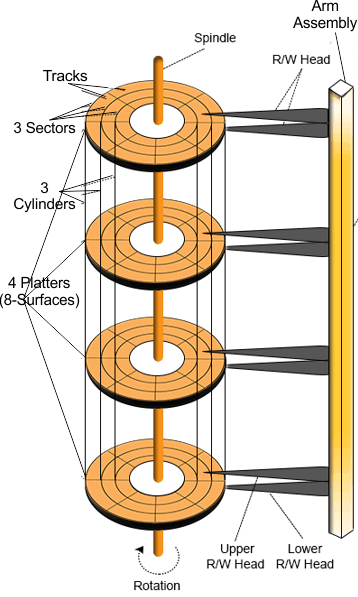
\includegraphics[width=0.7\linewidth]{OS Interaction with HDD.png}
    \caption{OS Interaction with HDD}
    \label{fig:OS and HDD}
\end{figure}